% Part 2 opening chapter: black-hole horizons. Carries the solid physics of the four G6 papers (read in full 2026-10-02):
%  BH Thermodynamics (25 Feb 2026), Information Paradox (Feb 2026), Bekenstein coefficient (Apr 2026).
% Checks: docs/verification/black_holes/BLACK_HOLES_CHECK.md; numbers: docs/verification/scripts/verify_virial_atoms_to_horizon.py.
% Interpretation (projection picture, paradox dissolution, cosmic censorship, particle fixed point) goes to Part 5.

\chapter{Black-hole horizons: Bekenstein, Hawking and the price of a bit}\label{ch:blackholes}

\section*{Overview}
IAM's Law (Chapter~\ref{ch:iams_law}) prices every classical record at $k_BT\ln2$ per bit on the nearest encoding surface. For a collapsed
mass the nearest surface is the black hole's own horizon, at the Hawking temperature; that horizon is the place in IAM this chapter reads.
Part~\ref{part:1} ended with the virial half: a system bound by $1/r$ holds half its binding energy as motion, and that half is the irreversible cost of binding. The
next rung of the ladder is the strongest binding there is. A black hole is a surface with a temperature and an entropy, and Landauer's principle can be
applied to it directly. When it is, the same half appears. This chapter sets out the thermodynamics of black-hole horizons, the rates at which they
take in and give out information, the relation between a black hole and the cold horizon of the universe, and where the famous factor $1/4$ in the
Bekenstein--Hawking entropy comes from. Chapter~\ref{ch:virial} then applies the same first law to the cosmic horizon.

\section{A horizon has a temperature and an entropy}
Bekenstein (1973)~\cite{Bekenstein1973} argued that a black hole must carry entropy proportional to its area; Hawking (1975)~\cite{Hawking1975} showed that it radiates thermally. For a
Schwarzschild black hole of mass $M$,
\begin{equation}
S_{\rm BH}=\frac{k_Bc^3A}{4G\hbar}=\frac{4\pi Gk_BM^2}{\hbar c},\qquad T_{\rm BH}=\frac{\hbar c^3}{8\pi Gk_BM},\qquad A=\frac{16\pi G^2M^2}{c^4}.
\end{equation}
Every causal horizon has a temperature set by its surface gravity $\kappa$,
\begin{equation}
T=\frac{\hbar\kappa}{2\pi k_Bc},
\end{equation}
with $\kappa=c^4/4GM$ for a black hole, $\kappa=cH$ for the de Sitter horizon of an expanding universe (Gibbons \& Hawking 1977~\cite{GibbonsHawking1977}), and $\kappa=a$ for an
observer with acceleration $a$ (Unruh 1976~\cite{Unruh1976}). The $2\pi$ is the period of the Euclidean time that makes the horizon smooth; it is the same in all three.

\begin{center}\small
\begin{tabular}{lcccc}
\hline
Mass ($M_\odot$) & $T_{\rm BH}$ (K) & $S_{\rm BH}$ (bits) & $\Gamma$ (bits\,s$^{-1}$) & $\tau_{\rm evap}$ (yr)\\\hline
1 & $6.17\times10^{-8}$ & $1.51\times10^{77}$ & $152.5$ & $2.10\times10^{67}$\\
10 & $6.17\times10^{-9}$ & $1.51\times10^{79}$ & $15.25$ & $2.10\times10^{70}$\\
$10^{6}$ & $6.17\times10^{-14}$ & $1.51\times10^{89}$ & $1.53\times10^{-4}$ & $2.10\times10^{85}$\\
$10^{9}$ & $6.17\times10^{-17}$ & $1.51\times10^{95}$ & $1.53\times10^{-7}$ & $2.10\times10^{94}$\\\hline
\end{tabular}
\end{center}

\section{The price of the horizon's bits}

\begin{figure}[htbp]\centering
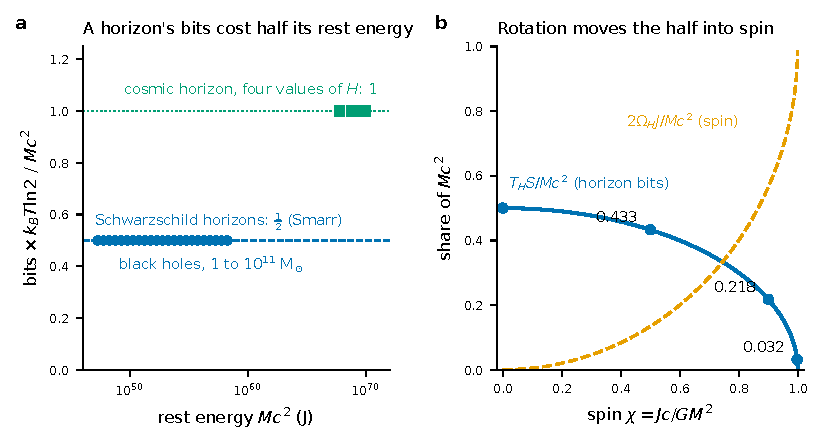
\includegraphics[width=\textwidth]{figures/part2/fig_smarr.pdf}
\caption{(a) The bits of a horizon, $N=S/(k_B\ln2)$, priced at its own temperature, divided by its rest energy. For Schwarzschild black holes from 1 to $10^{11}\,M_\odot$ the ratio is $1/2$ to machine precision ($|\Delta|<2\times10^{-16}$), the Smarr relation $T_{\rm BH}S_{\rm BH}=\tfrac12Mc^2$; for the cosmic horizon ($H_0=67.4$ to $10^4$\,km\,s$^{-1}$Mpc$^{-1}$) it is 1, $T_{\rm GH}S=M_Hc^2$. (b) Kerr: $T_{\rm BH}S_{\rm BH}/Mc^2=\sqrt{1-\chi^2}/2$ (0.500, 0.433, 0.218, 0.032 at $\chi=0$, 0.5, 0.9, 0.998) and the spin share $2\Omega_HJ/Mc^2$; the two sum to 1. \calc}\label{fig:smarr}
\end{figure}
Count the entropy in bits, $N=S_{\rm BH}/(k_B\ln2)$, and price each one at Landauer's minimum, $k_BT_{\rm BH}\ln2$. The total is
\begin{equation}
N\,k_BT_{\rm BH}\ln2=T_{\rm BH}S_{\rm BH}=\tfrac12Mc^2 ,
\end{equation}
exactly, for every mass: $0.5000000000$ for one solar mass, for the $4.3\times10^6\,M_\odot$ black hole at the centre of the Galaxy~\cite{Gillessen2009} and for the
$6.5\times10^9\,M_\odot$ black hole in M87~\cite{EHT2019}. In general relativity this is the Smarr relation $Mc^2=2T_{\rm BH}S_{\rm BH}$ (Smarr 1973~\cite{Smarr1973}; Bardeen, Carter \&
Hawking 1973~\cite{BardeenCarterHawking1973}). Read with Landauer's principle it says that half of a black hole's rest energy is the minimum cost of the information on its horizon --- the
same half that the virial theorem gives every $1/r$ system (Chapter~\ref{ch:virial_law}).

Rotation moves energy out of the horizon's bits and into spin. For a Kerr black hole with spin $\chi=Jc/GM^2$, $Mc^2=2T_{\rm BH}S_{\rm BH}+2\Omega_HJ$, and
\begin{equation}
\frac{T_{\rm BH}S_{\rm BH}}{Mc^2}=\frac{\sqrt{1-\chi^2}}{2}:\qquad 0.433\ (\chi=0.5),\quad 0.218\ (\chi=0.9),\quad 0.032\ (\chi=0.998).
\end{equation}
The half belongs to the non-rotating, fully relaxed horizon, as the virial half belongs to the relaxed bound system.

\section{How fast a horizon writes and erases}
In the black-body approximation a black hole radiates like any thermal surface,
\begin{equation}
P=\sigma_{\rm SB}AT_{\rm BH}^4=\frac{\hbar c^6}{15360\pi G^2M^2},
\end{equation}
with $\sigma_{\rm SB}=\pi^2k_B^4/(60\hbar^3c^2)$. The exact Hawking spectrum includes greybody factors and the count of particle species (Page 1976~\cite{Page1976}), which
change the numerical coefficient but not the scaling. Dividing the power by the cost per bit gives the rate at which the horizon's bits leave:
\begin{equation}
\Gamma=\frac{P}{k_BT_{\rm BH}\ln2}=\frac{c^3}{1920\,GM\ln2}\ \text{bits\,s}^{-1}.
\end{equation}
This is the first law of black-hole thermodynamics read in bits: $c^2|dM/dt|=T_{\rm BH}|dS_{\rm BH}/dt|$, so $\Gamma$ is the rate at which the horizon entropy
falls. The mass obeys $dM/dt=-P/c^2$, which integrates to
\begin{equation}
M(t)^3=M_0^3-\frac{\hbar c^4t}{5120\pi G^2},\qquad \tau_{\rm evap}=\frac{5120\pi G^2M_0^3}{\hbar c^4}.
\end{equation}
The entropy carried off grows as $S_{\rm BH,0}-S_{\rm BH}(t)=S_{\rm BH,0}[1-(1-t/\tau)^{2/3}]$: it reaches half of the initial horizon entropy at
$t=(1-2^{-3/2})\tau=0.646\,\tau$ and all of it at $\tau$. Smaller black holes are hotter and write faster.

\section{Two horizons: hot and cold}

\begin{figure}[htbp]\centering
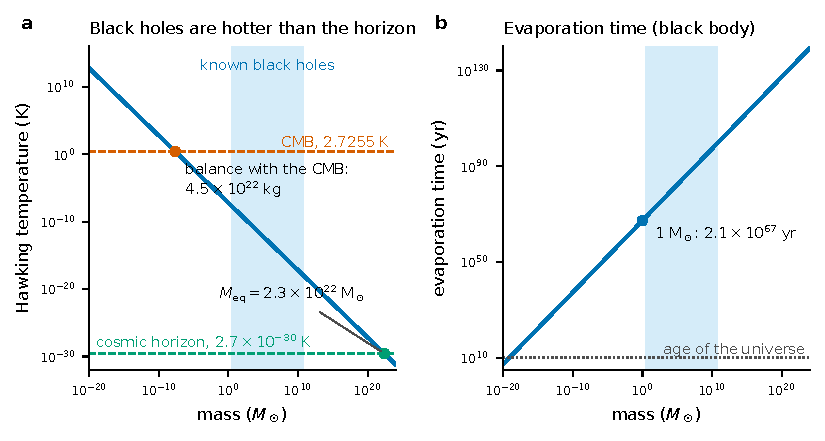
\includegraphics[width=\textwidth]{figures/part2/fig_bh_temperature.pdf}
\caption{(a) Hawking temperature against mass, with the CMB (2.7255\,K) and the cosmic horizon ($T_{\rm GH}=2.7\times10^{-30}$\,K, $H_0=67.4$). A black hole balances the CMB at $4.5\times10^{22}$\,kg and the horizon at $M_{\rm eq}=c^3/4GH_0=2.3\times10^{22}\,M_\odot$. Shaded: known black holes, 3 to $6.6\times10^{10}\,M_\odot$. (b) Black-body evaporation time $\tau_{\rm evap}=5120\pi G^2M^3/\hbar c^4$, $2.1\times10^{67}$\,yr for one solar mass; greybody factors change the coefficient, not the scaling. \calc}\label{fig:bh_temperature}
\end{figure}
The universe has its own horizon, at $c/H$, with the Gibbons--Hawking temperature $T_{\rm GH}=\hbar H/(2\pi k_B)=2.66\times10^{-30}$\,K today. A black hole is
in equilibrium with it only if $T_{\rm BH}=T_{\rm GH}$, at
\begin{equation}
M_{\rm eq}=\frac{c^3}{4GH}=2.32\times10^{22}\,M_\odot\quad(H_0=67.4\ \text{km\,s}^{-1}\text{Mpc}^{-1}),
\end{equation}
$1.3\times10^{22}$ at $z=1$ and $2.4\times10^{12}\,M_\odot$ at $z=10^6$. Every known black hole is far lighter (TON~618 is $6.6\times10^{10}\,M_\odot$~\cite{Shemmer2004}), so every
black hole is hotter than the cosmic horizon.

The sky a black hole actually sits in is not at $T_{\rm GH}$, though: it is filled with the cosmic microwave background at $T_{\rm CMB}=2.7255$\,K~\cite{Fixsen2009}. A
solar-mass black hole has $T_{\rm BH}=61.7$\,nK, $4.4\times10^{7}$ times colder, so today it absorbs about $(T_{\rm CMB}/T_{\rm BH})^4\approx4\times10^{30}$
times more radiation than it emits (equal-area black-body estimate) and grows. A black hole is in balance with the CMB at
\begin{equation}M_{\rm CMB}=\frac{\hbar c^3}{8\pi Gk_BT_{\rm CMB}}=4.5\times10^{22}\ \text{kg}\approx0.6\,\text{lunar masses};\end{equation}
only lighter holes, which no known process forms today, are net emitters now. Every stellar and supermassive black hole begins to lose mass only after
the expansion has cooled the CMB below its own temperature: for one solar mass the scale factor must grow another $4.4\times10^{7}$-fold (17.6 e-folds). From then on,
energy and entropy flow from the hot local horizon to the cold cosmic one at the rate $\Gamma$, over times of $10^{67}$ years and longer.

\section{When a horizon forms}
Thorne's hoop conjecture~\cite{Thorne1972} says a black hole forms when mass $M$ is compressed inside a circumference $4\pi GM/c^2$. At the Schwarzschild radius the
holographic bound $S/A\le k_B/(4\ell_P^2)$~\cite{Bousso2002} is met exactly:
\begin{equation}
\frac{4\pi Gk_BM^2/(\hbar c)}{4\pi(2GM/c^2)^2}=\frac{k_Bc^3}{4\hbar G}=\frac{k_B}{4\ell_P^2}.
\end{equation}
The two statements are one: the geometry of the hoop and the information capacity of the surface. Primordial black holes form by the standard
mechanism~\cite{Carr2010} during radiation domination, where electromagnetic interactions, not gravity, set the irreversible rate \interp.

\paragraph{How close a remnant is to its limit.} Every compact remnant is held up against gravity by a pressure that can only support so much
mass: electron degeneracy up to the Chandrasekhar mass~\cite{Chandrasekhar1931} ($1.44\,M_\odot$; $1.456\,M_\odot$ for $\mu_e=2$ from the constants alone), neutron
degeneracy and nuclear forces up to the Tolman--Oppenheimer--Volkoff limit~\cite{Tolman1939,OppenheimerVolkoff1939} (taken here as $\approx2.3\,M_\odot$; a recent multimessenger
inference gives $2.25^{+0.08}_{-0.07}\,M_\odot$~\cite{Fan2024}). On the same gauge as every other system in this book, $A$ is the remnant's mass over the typical remnant of its kind as built
(white dwarfs $0.6\,M_\odot$, the measured mean of $0.593\,M_\odot$ for DA white dwarfs~\cite{Kepler2007}; neutron stars $1.4\,M_\odot$), so $A=1$ sits in the middle. The far right is where the surface is
full: no pressure can hold, a horizon forms and the black hole begins (Fig.~\ref{fig:stargauge}).
\begin{center}\small\begin{tabular}{lccc}\toprule
remnant & mass ($M_\odot$) & $A$ & surface full at\\\midrule
the Sun's future white dwarf~\cite{Sackmann1993} & 0.54 & 0.90 & 2.40\\
Procyon B (wide binary)~\cite{Bond2015} & 0.59 & 0.99 & 2.40\\
Sirius B (wide binary)~\cite{Bond2017} & 1.02 & 1.70 & 2.40\\
IK Pegasi B (21.7-day binary)~\cite{Landsman1993} & 1.15 & 1.92 & 2.40\\
typical neutron star & 1.4 & 1.00 & 1.64\\
PSR J0740+6620~\cite{Fonseca2021} & 2.08 & 1.49 & 1.64\\\bottomrule
\end{tabular}\end{center}
A white dwarf that is isolated or in a wide binary has nothing to accrete, so it stays where it is; only a remnant that gains mass, from a close companion
as it evolves or from a collapsing core, moves right. What stops the star at the far right is ordinary physics, the pressure failing. What forms there is the object that holds the most entropy any
region of that size and energy can hold: a black hole saturates the Bekenstein bound~\cite{Bekenstein1981}. This is the one gauge in the book where the far-right line is
measured exactly; for cells the corresponding line is still to be measured (Chapter~\ref{ch:onegauge}, Part~\ref{part:5}) \openprob.
\begin{figure}[htbp]\centering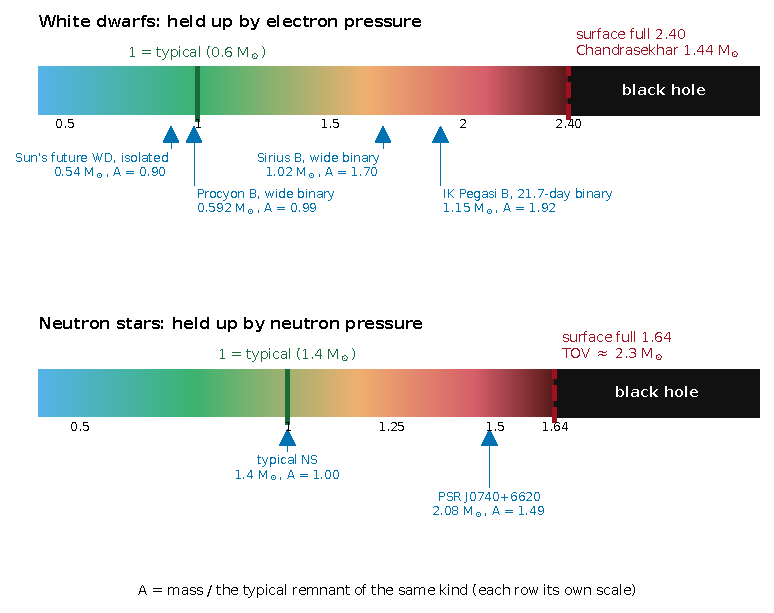
\includegraphics[width=\textwidth]{figures/part2/star_gauge.pdf}
\caption{Compact stars on the same gauge: mass over the typical remnant of the same kind ($0.6\,M_\odot$ white dwarfs, $1.4\,M_\odot$ neutron stars).
Dashed: the surface is full at the Chandrasekhar mass ($1.44\,M_\odot$, $A=2.40$) or the TOV limit ($\approx2.3\,M_\odot$, $A\approx1.64$); beyond,
a black hole. Each row has its own scale.}\label{fig:stargauge}\end{figure}

\section{Where the 1/4 comes from}
Jacobson (1995)~\cite{Jacobson1995} obtained the Einstein equations from $\delta Q=T\,\delta S$ on local Rindler horizons, with $T=\hbar\kappa/(2\pi k_Bc)$ and $S=\eta A$. The
Clausius relation holds for every null direction only if
\begin{equation}
\frac{\hbar\eta}{2\pi}=\frac{c^3}{8\pi G}\qquad\Longrightarrow\qquad\eta=\frac{c^3}{4\hbar G}=\frac{1}{4\ell_P^2}.
\end{equation}
The $1/4$ is the ratio of two geometric numbers: the $2\pi$ period of the Euclidean horizon (Bisognano \& Wichmann 1976~\cite{BisognanoWichmann1976}; Unruh 1976~\cite{Unruh1976}) and the $8\pi$ of the
field equations ($4\pi$ from Gauss's law in three dimensions, doubled by the trace structure of $G_{ab}$). Given Newton's constant, nothing else enters.
The same ratio gives one unit of entropy, $k_B$, per $4\ell_P^2$ of horizon; one bit takes $4\ln2\,\ell_P^2$. What thermodynamics cannot supply is why a smallest area $\ell_P^2=\hbar G/c^3$
exists at all; that is a question about the microstructure of spacetime.

\section{From the black hole to the universe}
A black hole's horizon carries entropy $A/4\ell_P^2$, sits at temperature $\hbar\kappa/2\pi k_Bc$, and holds half its mass-energy as the Landauer cost of its
bits. The horizon of the universe obeys the same first law. Jacobson and Cai \& Kim~\cite{Jacobson1995,CaiKim2005} showed that applying $-dE=T\,dS$ at the cosmic apparent horizon returns the
Friedmann equations. Chapter~\ref{ch:virial} adds to that first law the entropy written as matter decoheres, and the virial half fixes how much of the matter
density enters it: $\beta_m=\Omega_m/2$.

Seed masses of black holes cannot yet be computed from the information budget of collapse: the collapse entropy they require is not derived \openprob.
The formation of a horizon as the point where no outer surface can hold the records is taken up in Part~\ref{part:5} (Chapter~\ref{ch:theoryinterp}).
